\documentclass[11pt]{article}
\usepackage[margin=1in]{geometry}
\usepackage{amsmath,amssymb}
\usepackage{lmodern}
\usepackage[T1]{fontenc}
\usepackage{enumitem}
\usepackage{microtype}
\usepackage{tikz}
\usetikzlibrary{arrows.meta,angles,quotes,calc,decorations.pathreplacing}

\title{2013 F=ma Exam Review}
\author{Nathan P.}
\date{February 1, 2026}

\begin{document}
\maketitle

\section*{Problem 3}
A is true because $\sin 2\theta\le 1$ and $R=v^2\sin 2\theta/g$, so $gR\le v^2$.
If $v$ increases with $R$ held fixed, the min value of $t$ decreases because you can shoot at a smaller angle faster, and the max value of $t$ increases because you can shoot at a larger angle. Overall, increasing $v$ expands the range of time values.
If $R$ increases with $v$ held fixed, the min value of $t$ increases because you need to shoot at a higher angle, and the max value of $t$ decreases because you need to shoot at a less steep angle. Overall, increasing $R$ narrows the range of time values.

\section*{Problem 4}
Balance torques about the hinge.

\section*{Problem 9}
Yes, the initial $p=Ft$, but that's not an option.
\[
x=v_{\text{avg}}t,\qquad t=\frac{x}{v_{\text{avg}}}=\frac{x}{v/2}=\frac{2x}{v},\qquad Ft=\frac{2Fx}{v}.
\]
Or: $K_i=\tfrac12mv^2=\tfrac12pv$, so $p=2K_i/v$, and from the previous problem $K_i=Fx$, so $p=2Fx/v$.

\section*{Problem 12}
Don't skip writing out the force equations for this one. The frictionless fluid contributes to the mass but not to the rotational inertia about the com, because it's not rotating.
\[
2Mg\sin\theta-f=2Ma,\qquad fR=I\alpha,\qquad I=\tfrac23MR^2\ \text{(only the $M$ of the shell rotates)},\qquad \alpha=\frac aR
\]
(roll without slip), so $f=\tfrac23Ma$. Proceed to solve for $a$.

\section*{Problem 13}
For the rings to be part of Saturn, $v=r\omega$ (they have to rotate at the same $\omega$). Don't mix up the $\omega$ of the planet's rotation and the $\omega$ of an orbit: $v^2\propto 1/R$ is the result for orbiting satellites, not for something that's part of the rigid rotating body. For the rings to be part of Saturn, $v\propto R$, that's it; the $\omega$ of the planet's rotation is just some constant.

\section*{Problem 15}
Torque balance. Set a $\theta$; it'll cancel.
The buoyant force acts at the midpoint of the portion of the rod under water.
$V_{\text{sub}}/V=L_{\text{sub}}/L$ (the cross-sectional areas cancel).

\begin{center}
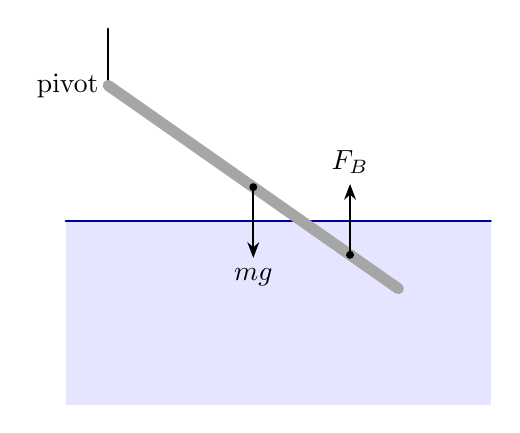
\begin{tikzpicture}[scale=0.9, line cap=round, line join=round, >={Stealth[length=2mm]}]
  \fill[blue!10] (-0.6,-2.6) rectangle (5.4,0);
  \draw[thick, blue!60!black] (-0.6,0) -- (5.4,0);
  \coordinate (P) at (0,{5*(2/3)*sin(35)});
  \coordinate (E) at ($(P)+(-35:5)$);
  \draw[thick] (P) -- ++(0,0.8);
  \fill (P) circle (2pt) node[left] {pivot};
  \draw[line width=4pt, gray!70] (P) -- (E);
  % midpoint of the rod and midpoint of the submerged part
  \coordinate (M) at ($(P)!0.5!(E)$);
  \coordinate (W) at ($(P)!{2/3}!(E)$);
  \coordinate (B) at ($(W)!0.5!(E)$);
  \draw[->, thick] (M) -- ++(0,-1.0) node[below] {$mg$};
  \draw[->, thick] (B) -- ++(0,1.0) node[above] {$F_B$};
  \fill (M) circle (1.6pt);
  \fill (B) circle (1.6pt);
\end{tikzpicture}
\end{center}

\section*{Problem 18}
Closed system $\to$ $\Delta p=0$, $v_{cm}$ is constant $=0$, so $v=0$, so $\Delta x_{cm}=0$. $\Delta L$ is also conserved.
Remember: $L$ about a point is $mv$ times the lever arm.

\section*{Problems 23 \& 24}
Set up the simple energy and force equations, and solve. The answer isn't automatically in the same format, hinting that you need the relation between $h$ and $H$.

\section*{Problem 25}
The first sentence lets you find an expression for $\mu$.
Read carefully: $P$ is a force, not power, in this problem.
Because the force is horizontal, there is a component perpendicular to the incline, so you must account for greater friction: $\mu(W\cos\theta+P\sin\theta)$. Carry out the algebra to solve for $P$ in terms of $W$.

\end{document}
